
耦合和内聚是软件的两个术语。来看看它们的含义,以及它们之间的关系。


\subsubsubsection{1.8.1\hspace{0.2cm}耦合}

耦合是软件单元对其他单元依赖的程度。具有高耦合的单元依赖于许多其他单元,所以耦合度越低越好。

如果一个类依赖于另一个类的私有成员,则它们是紧密耦合的。第二个类的变化意味着第一个类也需要改变,这就是为什么高耦合不是一个理想的状态。

为了弱化耦合,可以考虑为成员函数添加参数,而不是直接访问其他类的私有成员。

紧密耦合的另一个例子是依赖倒置中的\texttt{Project}和\texttt{developer}类的第一个实现。如果添加另一个开发者类型会发生什么:


\begin{lstlisting}[style=styleCXX]
class MiddlewareDeveloper {
public:
	void developMiddleware() {}
};

class Project {
public:
	void deliver() {
		fed_.developFrontEnd();
		med_.developMiddleware();
		bed_.developBackEnd();
	}

private:
	FrontEndDeveloper fed_;
	MiddlewareDeveloper med_;
	BackEndDeveloper bed_;
};
\end{lstlisting}

看起来不仅是添加了\texttt{MiddlewareDeveloper}类,还必须修改\texttt{Project}类的公共接口。所以它们是紧密耦合的,并且\texttt{Project}类的实现破坏了OCP。再来看看如何使用依赖倒置将相同的修改应用于实现的:


\begin{lstlisting}[style=styleCXX]
class MiddlewareDeveloper {
public:
	void develop() { developMiddleware(); }
	
private:
	void developMiddleware();
};
\end{lstlisting}

不需要更改\texttt{Project}类,所以现在这些类是松散耦合的,所需要做的就是添加\texttt{MiddlewareDeveloper}类。以这种方式构造代码就能保证更小范围的重构、更快的开发和更容易的测试,所有这些都需要更少的代码,并且更容易维护。使用的新类,只需要修改调用代码:

\begin{lstlisting}[style=styleCXX]
using MyProject = Project<FrontEndDeveloper, MiddlewareDeveloper, BackEndDeveloper>;
auto alice = FrontEndDeveloper{};
auto bob = BackEndDeveloper{};
auto charlie = MiddlewareDeveloper{};
auto new_project = MyProject{{alice, charlie, bob}};
new_project.deliver();
\end{lstlisting}

这显示了类级别上的耦合。两个服务之间,可以通过引入消息队列等技术来实现低耦合。这样,服务就不会直接相互依赖,并且只依赖于消息格式。如果有一个微服务架构,常见的错误是让多个服务使用相同的数据库。因为无法修改数据库模式,从而不影响使用微服务,进而导致了服务之间的耦合。

\subsubsubsection{1.8.2\hspace{0.2cm}内聚}

内聚是软件单元之间的关联度。在高度内聚的系统中,同一模块中组件所提供的功能是紧密相关的,这感觉这些组件是一个整体。

在类级别上,一个方法操作的字段越多,它与类的内聚性就越强。最常见的低内聚数据类型,是那些大型单数据类型。当类中有太多内容时,就会缺乏内聚性,也会破坏SRP。这使得这些类很难维护,并且容易出现Bug。

较小的类也可能不具有内聚性,考虑下面的示例。这可能看起来没什么,但真实的场景中,通常是数百甚至数千行:

\begin{lstlisting}[style=styleCXX]
class CachingProcessor {
public:
	Result process(WorkItem work);
	Results processBatch(WorkBatch batch);
	void addListener(const Listener &listener);
	void removeListener(const Listener &listener);
	
private:
	void addToCache(const WorkItem &work, const Result &result);
	void findInCache(const WorkItem &work);
	void limitCacheSize(std::size_t size);
	void notifyListeners(const Result &result);
	// ...
};
\end{lstlisting}

可以看到处理器实际上执行三种类型的工作:实际工作、缓存结果和管理监听器。在这种情况下,增加内聚的常见方法是提取一个或多个类:

\begin{lstlisting}[style=styleCXX]
class WorkResultsCache {
public:
	void addToCache(const WorkItem &work, const Result &result);
	void findInCache(const WorkItem &work);
	void limitCacheSize(std::size_t size);
private:
	// ...
};

class ResultNotifier {
public:
	void addListener(const Listener &listener);
	void removeListener(const Listener &listener);
	void notify(const Result &result);
private:
	// ...
};

class CachingProcessor {
public:
	explicit CachingProcessor(ResultNotifier &notifier);
	Result process(WorkItem work);
	Results processBatch(WorkBatch batch);
private:
	WorkResultsCache cache_;
	ResultNotifier notifier_;
	// ...
};
\end{lstlisting}

现在,每个部分都是由独立的、内聚的实体完成的。重用它们没什么问题,也不会有太多麻烦。甚至将它们变成模板类也不需要太多的工作,测试这样的类也会更容易。

将其置于组件或系统级别上会非常简单——设计的每个组件、服务和系统都应该简洁,专注于做一件事,并且把它做好:

\begin{center}
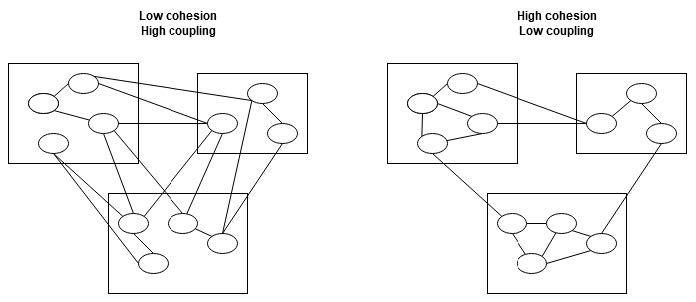
\includegraphics[width=0.9\textwidth]{content/1/chapter1/images/2.jpg}\\
图1.2 - 耦合与内聚
\end{center}

低内聚和高耦合通常与难以测试、重用、维护甚至理解的软件相应的关联性,因此它缺乏软件中需要的质量属性。

这两个术语经常同时出现,通常一个特征影响另一个特征,不管是功能、类、库、服务,甚至是整个系统。通常情况下,单体服务是高度耦合和低内聚的,而分布式服务则处于另一个极端。

现在让我们总结一下所了解到的知识。